\newpage
\section{Overview}
\label{chapter1}

\subsection{SafeDM description}
\label{descrption_subsec}

SafeDM is a hardware Diversity Monitor that quantifies the diversity of each redundant processor to guarantee that CCF will not go unnoticed, and without needing to deploy lockstepped cores. SafeDM takes advantage of the fact that diversity naturally exists due to the complexity of the system to develop the safety concept. Each cycle SafeDM computes one signature per core summarizing their internal state. Both signatures are compared and if they coincide, lack of diversity is reported.

SafeDM is instantiated in the SoC as an APB slave\footnote{Based on AMBA 2.0 specification}. SafeDM raises an output each cycle that diversity is missed between cores. SafeDM also has an internal counter that is increased by one each cycle that there is lack of diversity. The value of this counter can be retrieved through the APB bus reading the appropriate register. SafeDM only reports a lack of diversity in the system and it is up to the user to determine the proper actions in the event of missing diversity.


%TODO:change image
\begin{figure}[H]
	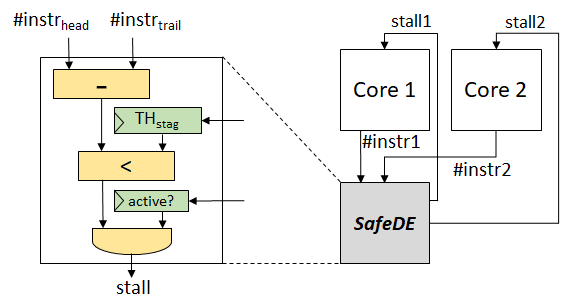
\includegraphics[keepaspectratio,width=\columnwidth]{img/safede}
        \caption{SafeDM simplified scheme.} %Maybe change it
	\label{fig:simplified_scheme}
\end{figure}
Figure \ref{fig:simplified_scheme} shows a simplified scheme of SafeDM connected to two redundant processors. Internally, SafeDM generates two different signatures: instruction and data signatures. Some internal signals from the pipeline and the register file are required to calculate those signatures.

The signatures are generated by storing the last instructions processed in the decode stage and the last values read from the register file ports in FIFOs. In image ... we can see an example: \textcolor{red}{add picture}

SafeDM offers some advantages in comparison to lockstep approaches:
\begin{itemize}
	\item \textbf{Performance:} Classical tight-lockstep approach employs two cores that are seen as one by the user, thus halving the performance. A pair of redundant cores monitored by SafeDM can execute different tasks at any time.
	\item \textbf{Instructions stream:} Other lockstep approaches as light\-lockstep avoid the performance penalty of the tight\-lockstep but require identical instructions streams. This prevents this solution from executing parallel applications or handling the system's inputs and outputs. SafeDM overcomes this limitation.
    \item \textbf{Low intrusiveness:} SafeDM can be implemented in a SoC performing only a few modifications in the design. SafeDM only needs a few signals to calculate the signatures.
\end{itemize}



\subsection{Licensing}

This BSC IP core module is freely provided under the terms of the MIT License.



\hspace{5cm}
